%\section{Understanding and Modeling Transient Server Preemptions}
%\section{Modeling the Dynamics of Transient Server Preemptions}
%\section{Preemption Dynamics of Transient Cloud Servers}
\vspace*{\subsecspace}
\section{Constrained Preemptions of Google Preemptible VMs}
\label{sec:preemption-dynamics}

%Understanding the nature and dynamics of transient cloud servers such as their preemption frequency is a prerequisite to understand and improve the performance of applications.

%This is presumably in the background 
\eat{In order to understand and improve the performance of applications running on transient cloud servers, we must understand the nature and dynamics of their preemptions.
The preemption characteristics are governed by the supply of surplus resources, the demand for cloud resources, and the resource allocation policies enforced by the cloud operator.
Therefore, in this section, we present empirical and analytical models to help us understand the nature of preemptions. 
}

To measure and improve the performance of applications running on transient cloud servers, it is critical to understand the nature and dynamics of their preemptions. 
%The preemption characteristics are governed by the supply of surplus resources, the demand from applications, and resource allocation policies of the cloud operator.
In this section, we present empirical analysis of preemptions of Google Preemptible VMs, and develop new probabilistic models of their preemption rates.  
%that describe these characteristics and enable an intuitive understanding of the nature of preemptions. 


% Transient cloud servers, by their very nature have limited availability and are frequently preempted.
% These preemptions are akin to fail-stop failures, and are often preceeded by a small advance warning (few seconds) to allow for graceful shutdowns.

% Since preemptions can impact the availability, performance, and cost of running applications, in this section, we examine their preemption characteristics.
% This modeling is important, because having a model of the availability can be useful in the context of predicting the running times of applications.
% Cloud providers offer a large number of servers of different configurations and types.
% Since transient server availability is fundamentally tied to supply and demand, the availability of servers of different types can be significantly different. 
% Thus, selecting the ``right'' server type is crucial for minimizing the overall costs. 



%\cite{alicloud-spot, packet-spot}

%\subsection{Empirical model of preemptions}
%\subsection{Empirical preemption behavior}
\vspace*{\subsecspace}
\subsection{Empirical Study Of Preemptions}

% The preemptions of transient servers need not be related to their price.

To understand the nature of temporally constrained preemptions, we conducted the first empirical study of Google's Preemptible VMs, that have a fixed price and a maximum 24 hour lifetime.
Our empirical study is necesitated by the fact that the cloud operator (Google) does not disclose any other information about the preemption rates, and thus relatively little is known about the preemptions (and hence the performance) of these VMs.


We launched more than 1,500 Google Preemptible VMs of different types over a two month period (Feb--April 2019), and measured their time to preemption (i.e., their useful lifetime).\footnotemark

\footnotetext{We will release the complete preemption dataset for further analysis.} %Weaksauce 


\begin{figure}
  \centering 
  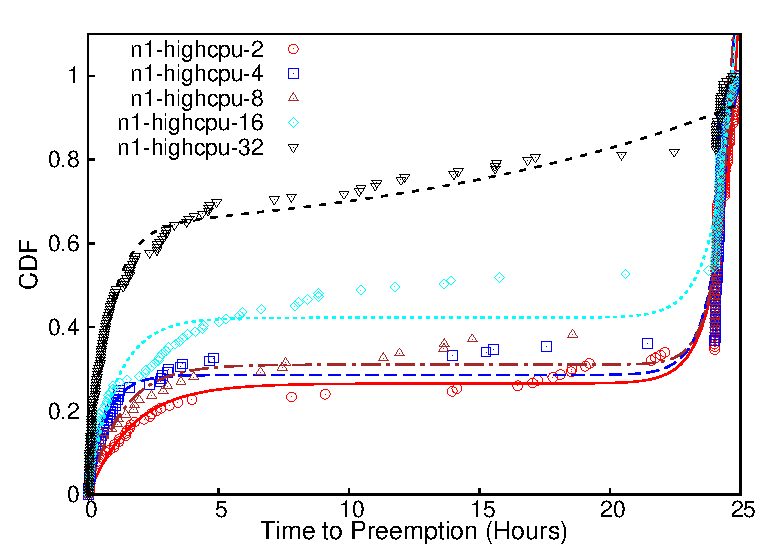
\includegraphics[width=0.4\textwidth]{../graphs/scispot-fig-vm-types.eps}
  \caption{Preemption characteristics of different VM types. Larger VMs are more likely to be preempted.}
  \label{fig:cdf-comparison}
    \vspace*{\myfigspace}
\end{figure}

\begin{figure}
  \centering 
  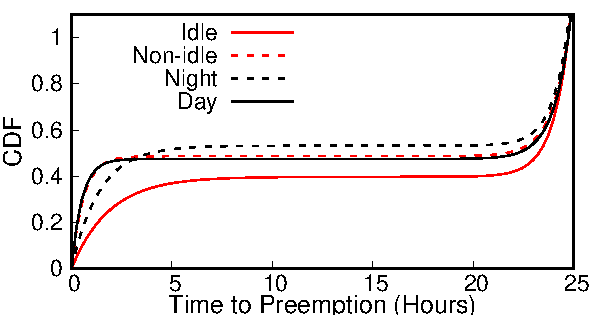
\includegraphics[width=0.35\textwidth]{../gnuplot_analysis/time-breakdown.pdf}
      \vspace*{\myfigspace}
  \caption{Variations due to time of day and workload.}
  \label{fig:time-breakdown}
    \vspace*{\myfigspace}
\end{figure}



A sample of over 100 such preemption events are shown in Figure~\ref{fig:gcp1}, which shows cumulative distribution function (CDF) of the VM lifetimes of the \texttt{n1-highcpu-16} VM in the \texttt{us-east1-b} zone. 
%enter the type of VM for which the data is shown
Note that the cloud operator (Google) caps the \emph{maximum} lifetime of the VM to 24 hours, and all the VMs are preempted before that limit. 

\noindent \textbf{Observation 1:} \emph{The lifetimes of VMs are not uniformly distributed, but have three distinct phases.}

\noindent In the first (initial) phase, characterized by VM lifetime $t\in [0, 3]$ hours, we observe that many VMs are quickly preempted after they are launched, and thus have a steep rate of failure (derivative of the CDF) initially.
%; the rate of failure or preemptions can be obtained by taking the derivative of the CDF. 
In the second phase, VMs that survive past 3 hours enjoy a relatively low preemption rate over a relatively broad range of lifetime (characterized by the slowly rising CDF in Figure~\ref{fig:gcp1}).
The third and final phase exhibits a steep increase in the number of preemptions as the preemption deadline of 24 hours approaches.
The overall rate of preemptions is ``bathtub'' shaped as shown in the inset of Figure~\ref{fig:gcp1}.
%\it I think we should show the probability plot to exhibit the bath tub shape

%The preemption rate is ``bath tub'' shaped, with VMs that survive past 3 hours enjoying a relatively low preemption rate, and finally a steep increase in the number of preemptions as the preemption deadline (24 hours) approaches. 


\noindent \textbf{Observation 2:} \emph{The preemption behavior, imposed by the constraint of the small 24 hour  lifetime, is substantially different from conventional failure characteristics of hardware components and even EC2 spot instances.}

\noindent In ``classical'' reliability analysis, the rate of failure  usually follows an exponential distribution $f(t) = \lambda e^{-\lambda t}$, where $\lambda=1/\text{MTTF}$.
Figure~\ref{fig:gcp1} shows the CDF ($=1-e^{-\lambda t}$) of the exponential distribution when fitted to the observed preemption data, by finding the distribution parameter $\lambda$ that minimizes the least squares error.
The classic exponential distribution is unable to model the observed preemption behavior because it assumes that the rate of preemptions is independent of the lifetime of the VMs, i.e., the preemptions are \emph{memoryless}.
%The primary reason is that the exponential distribution assumes that the \vj{the rate of preemptions is independent of the lifetime of the VMs} (preemptions are \emph{memoryless}), which does not hold true when there is a fixed upper bound on the lifetime, as is the case for Google Preemptible VMs. \vj{In other words, the conventional approach is insufficient to model constrained preemption dynamics.}
%We attribute this deficiency to the central assumption made in the underlying reliability theory principles that leads to the classical exponential distribution: the rate of preemptions is independent of the lifetime of the VMs, in other words, the preemptions are \emph{memoryless}.
This assumption breaks down when there is a fixed upper bound on the lifetime, as is the case for Google Preemptible VMs, and the conventional approach becomes insufficient to model this constrained preemption dynamics. 

\noindent \textbf{Observation 3:} \emph{The bathtub shaped preemption behavior is a general, universal characteristic of Preemptible VMs.}

In general, the preemption dynamics of a VM is determined by the supply and demand of VMs of that \emph{particular} type.
Thus, our empirical study looked at preemptions of VMs of different sizes, in different geographical zones, at different times of the day, and running different workloads (Figure).
In all cases, we find that the preemption behavior is bathtub shaped.
We argue that this is not a coincindence, but may be a result of practical and fundamental outcomes of cluster management policies. 

While the actual preemption policy is up to the cloud operator,  we argue that the bathtub behavior has benefits for applications. 
%The bathtub behavior results in a high rate of failure initially. 
For applications that do not incorporate explicit fault-tolerance, early preemptions result in less wasted work than if the preemptions were uniformly distributed over the 24 hour interval.
Furthermore, the low rate of preemptions in the middle periods allows jobs that are smaller than 24 hours to finish execution with only a low probability of failure.
We compare job performance with bathtub shaped preemptions vs. uniform preemption rates in Section Evaluation.


In addition to being beneficial to applications, we also conjecture that the bathtub behavior is a \emph{fundamental} characteristic of any system where events are randomly distributed in a finite interval.
Intriguingly, we can analyze temporally constrained preemptions through a statistical mechanics framework, and we elaborate on this connection later in this Section. 


\noindent \textbf{Observation 4:}\emph{ Larger VMs have a higher rate of failure.}

\noindent Figure~\ref{fig:cdf-comparison} shows the preemption data from five different types of VMs in the Google Cloud \texttt{n1-highcpu-\{2,4,8,16,32\}}, where the number indicates the number of CPUs.
All VMs are running in the \texttt{us-central1-c} zone. 
Larger VMs require more computational resources (such as CPU and memory), and when the supply of resources is low, the cloud operator can reclaim a large amount of resources by preempting larger VMs.
This observed behavior aligns with the guidelines for using preemptible VMs that suggests the use of smaller VMs when possible~\cite{preemptible-documentation}. 

\noindent \textbf{Observation 5:} \emph{Preemptions exhibit diurnal variations, and are also affected by the workload inside the VM.}

\noindent From Figure~\ref{fig:time-breakdown}, we can see that VMs have a slightly longer lifetime during the night (8 PM to 8 AM) than during the day.
This is expected because fundamentally, the preemption rates are higher during periods of higer demand. 

We also notice that completely idle VMs have longer lifetimes than VMs running some workload.
Presumably, this could be a result of the lower resource utilization of idle VMs being more amenable to resource overcommitment, and result in lower preemptions. 

%being more amenable to resource overcommitment, and therefore don

%%%%%%%%%%%%%%%%%%%%%%%%%%%%%%%%%%%%%%%%%%%%%%%%%%%%%%%%%%%%%%%%%%%%%%

\vspace*{\subsecspace}
\subsection{Failure Probability Model}
\label{subsec:analytical-model}

We now develop an analytical model for preemption dynamics that is faithful to the empirically observed data and provides a basis for developing running-time and cost-minimizing optimizations. % presented in Section~\ref{sec:design}. 
%
To describe failures (preemptions) that are not memoryless (i.e., increasing or decreasing failure rate over time), the classic Weibull distribution with CDF $F(t)=1-e^{-(\lambda t)^k}$ is often employed. However, the Weibull distribution is also unable to fit the empirical data (Figure~\ref{fig:gcp1}). 
We also analyze other distributions used for modeling bathtub failures from reliability and actuarial theory in Figure \textbf{XXX}.




The non-trivial bathtub-shaped failure rate of Google preemptible VMs (Figure~\ref{fig:gcp1}) requires models that capture the sudden onset of  the rise in preemptions near the deadline. 
%which imposes a dynamics that is more akin to a constrained dynamics problem as opposed to dynamics characterized with a gradually rising failure rate.
We can see from the \textbf{QQ plots} that existing distributions are unable to capture all the phases of the preemptions. 



This is especially important from a policy design perspective, as the ``phase changes'' in preemption behavior can greatly affect the failure probability and performance of applications.
Our new model, informed by the cumulative distribution of lifetimes that has multiple distinct temporal phases, addresses this need.


The key assumption underlying our model is the presence of two distinct failure processes.
%that give rise to a new probability distribution characterizing the preemptions and the observed CDF, and ensure the dependence of the rate of failure on the VM lifetime. 
The first process dominates over the initial temporal phase and yields the classic exponential distribution that captures the high rate of early preemptions.
The second process dominates over the final phase near the 24 hour maximum VM lifetime and is assumed to be characterized by an exponential term that captures the sharp rise in preemptions that results from this constrained lifetime. 
%Generally, these two processes jointly determine the dynamics of preemptions during the middle phase where a relatively constant or a slowly rising number of preemptions with time is observed.
%; in practice, based on the fits to the empirical data, we observe the first process to dominate over the second during this phase as well. 

%The first two phases are reasonably captured by the classic exponential distribution. In order to model the overall observed empirical CDF, we add another term that captures the failure process near the 24 hour maximum VM lifetime,  and construct a \emph{new} probability distribution. 
%
%we develop a \emph{new} probability distribution that is composed by blending two failure processes that act on different temporal phases over the 24 hour maximum lifetime of the VMs. 
%
%We write the general form of our blended preemption CDF as follows:

Based on these observations, we propose the following general form for the CDF:

\vspace*{\subsecspace}
\begin{equation}
  \label{eq:blend1}
  \boxed{
  \mathscr{F}\left(t\right) = A\left(1-e^{-\frac{t}{\tau_1}} + e^{\frac{t-b}{\tau_2}}\right)}
  \end{equation}
\noindent where $t$ is the time to preemption, $1/\tau_1$ is the rate of preemptions in the initial phase, $1/\tau_2$ is the rate of preemptions in the final phase, $b$ denotes the time that characterizes ``activation'' of the final phase where preemptions occur at a very high rate, and $A$ is a scaling constant.
In practice, typical fit values yield $b \approx 24$ hours, and $\tau_2 \approx 1$ hour, which ensures that our proposed distribution meets the initial condition $\mathscr{F}(0) \approx 0$.

%of  0 $\approx 0$ premptions.
%used to scale the CDF to ensure that the initial conditions ($F(0)=0$) are met.

For most of its life, a VM sees failures according to the classic exponential distribution with a rate of failure equal to $1/\tau_1$ -- this behavior is captured by the $1-e^{-t/\tau_1}$ term in Equation~\ref{eq:blend1}. 
%However, this does not capture the finite lifetime of the VM imposed by the cloud operator.
As VMs get closer to their maximum lifetime imposed by the cloud operator, they are reclaimed (i.e., preempted) at a high rate $1/\tau_2$, which is captured by the second exponential term, $e^{(t-b)/\tau_2}$ of Equation~\ref{eq:blend1}. 
Shifting the argument ($t$) of this term by $b$ ensures that the exponential reclamation is only applicable near the end of the VM's maximum lifetime and does not dominate over the entire temporal range. 
%As noted before, $1/\tau_2$ is the rate of this reclamation. 

The analytical model and the associated  distribution function $\mathscr{F}$ introduced above provides a much better fit to the empirical data (Figure~\ref{fig:gcp1}) and captures the different phases of the preemption dynamics through parameters $\tau_1, \tau_2, b$, and $A$. These parameters can be obtained for a given empirical CDF using least squares function fitting methods. The failure or preemption rate can be derived from this CDF as:
\begin{equation}
  \label{eq:failrate}
    \vspace*{\eqnspace}
f(t) = \dfrac{d \mathscr{F}(t)} {dt} = A \left(\dfrac{1}{\tau_1}e^{-t/\tau_1} + \dfrac{1}{\tau_2}e^{\frac{t-b}{\tau_2}}\right).
\end{equation}
$p(t)$ vs. $t$ yields a bathtub type failure rate function for the associated fit parameters (inset of Figure~\ref{fig:gcp1}).
%In the next section, we use this analytical model for optimizing cloud resource selection to run scientific computing applications at low cost and shorter running (turnaround) times.


In the absence of any prior work on constrained preemption dynamics, our aim is to provide an interpretable model with a minimal number of parameters, that provides a sufficiently accurate characterization of observed preemptions data. 
%As is evident from Figure~\ref{fig:gcp1}, our model shows deviations from the data near the halfway point within the 24 hour lifetime. 
Further generalization of this model to include more failure processes would introduce more parameters and reduce the generalization power.
Exploring other approaches of modeling bathtub-type failure rates (e.g., exponential Weibull distributions) \cite{mudholkar1993exponentiated,crevecoeur1993model} is part of our future work. 


\subsubsection{Reliability Analysis}

We now look at constrained preemptions through the framework of reliability theory.
Based on the empirically observed bathtub shape, we analyze the hazard rate and the expected lifetime that is useful for developing Transiency-mitigation policies.

Our analytical model also helps crystallize the differences in VM preemption dynamics, by allowing us to easily calculate their expected lifetime. 
More formally, we define the expected lifetime of a VM of type $i$, as: 
\begin{equation}
  \label{eq:expected-lifetime}
E[L_i] =  \int_{0}^{24} t {p_i}(t)~dt =  -A(t+\tau_1)e^{-t/\tau_1} + A(t-\tau_2) e^{\frac{t-b}{\tau_2}} \biggr\rvert_{0}^{24}
\end{equation}
where $p_i(t)$ is the rate of preemptions of VMs of type $i$ (Equation~\ref{eq:failrate}).
%= \dfrac{d \mathscr{F}(t)} {dt} = A \left(\dfrac{1}{\tau_1}e^{-t/\tau_1} + \dfrac{t-b}{\tau_2}e^{\frac{t-b}{\tau_2}}\right) $ 
%
%Since preemptions require restarting a job and increase the job completion time, it may be more prudent to select transient VMs with higher expected lifetimes.
We use the analytically derived expected lifetimes of VMs of different types in \sysname when selecting the ``best'' VM type for a given bag of jobs. This server selection is a key part of \sysname design. 



Based on our CDF, the survival rate is $S (t) = 1- F(t) = e^{- r_1 t} - e^{r_2 (t - b)}$.
The hazard rate is defined as $\lambda(t) = \frac{S(t)}{f(t)}$.
Note that the hazard rate is constant for exponential distributions.

In our case, we can compute $\lambda(t) = \dfrac{- r_1 e^{- r_1 t} - r_2 e^{r_2 (t -
    b)}}{e^{- r_1 t} - e^{r_2 (t - b)}}$

Simplifying this expression leads to:

$\lambda = r_2 + \bar{r} \left( \dfrac{1}{1 - e^{- r_2 b} e^{\bar{r} t}}
\right) = \dfrac{r_1 + r_2 e^{- r_2 b} e^{\bar{r} t}}{1 - e^{- r_2 b}
e^{\bar{r} t}}$

Here, $\bar{r} = r_1 + r_2$, ie., the sum of the two failure rate constants.

Intuitively, for constrained preemptions, we expect the hazard rate to rise near the deadline, which is what the denominator accomplishes.
Because of the hard deadline, we get an exponential increase in the hazard rate.
However because the sudden reclamation only applies towards the very end of the deadline, our activation time parameter ($b$) helps delaying this sudden onset of preemptions. 



% We emphasize that our motivation is to develop an interpretable \emph{minimal} model that provides a sufficiently accurate description of the observed constrained preemption dynamics of Google VMs with a minimal number of meaningful parameters. 
% As is evident from Figure~\ref{fig:gcp1}, $\mathscr{F}$ shows deviations from the data near the halfway point within the 24 hour lifetime.
% Further generalization of this model to include more failure processes, which would introduce more parameters, or exploring other approaches of modeling bathtub-type failure rates (e.g., exponential Weibull distributions) \cite{mudholkar1993exponentiated,crevecoeur1993model} may yield alternate model descriptions that capture the data with higher accuracy.


%PXXX part of future work? 

%characterized by failure rates and activation times (like $b$). 
%and reduce the predictive power and simplicity of the model. 
%We also note that approaches (e.g., exponential Weibull distributions) to model bathtub-type failure rates have been proposed in the literature  \cite{mudholkar1993exponentiated,crevecoeur1993model}.
%These methods did not perform better than our model resulting in parameter variables and values that were relatively difficult to interpret; this could likely be due to the unique constraint-driven failures in preemption dynamics as opposed to aging-related increasing failure rate considered in previous work. 

\subsection{Connection to Statistical Mechanics}

In addition to empirically-informed reliability models for preemptions, we also seek to understand \emph{why} their distribution is bathtub shaped in order to provide a mechanistic understanding of preemptions and enhance the model interpretability and generalizability. 
%Our key insight is that the problem of analyzing constrained preemptions can be ``mapped'' to an equivalent problem in statistical mechanics of a physical system, and we can use the theoretical and analytical framework of statistical mechanics to develop a broader understanding of preemptions. 
%This connection to statistical mechanics is given below. 
To this end, we propose to ``map'' the problem of constrained preemptions to an equivalent problem of constrained many particle physical systems that can be analyzed employing the general theoretical framework of statistical mechanics.


A simple mapping can be established by assuming that the cluster management policy requires mutually exclusive preemptions.
This assumption helps cluster management by serializing VM preemptions and making cluster operations easier, and it reduces the challenges associated with reacting to simultaneous preemptions. The preemption events become hard particles that cannot overlap. The probability distribution of $N$ constrained preemption events gets mapped to the density of $N$ randomly distributed particles confined in a 1-dimensional interval of length $L$ (analogous to 24 hours). 
The particle size is equivalent to the length of the critical section, which is related to the preemption warning (30 seconds for Google PVMs).
Finding the distribution of non-overlapping (i.e., hard) particles is a central problem in statistical mechanics [5].
%Interestingly, the distribution of particles in a confined interval can be obtained analytically via the exact closed-form expression of the so-called partition function (a common statistical mechanical quantity useful for obtaining the microscopic understanding of macroscopic phenomena).
This distribution is \emph{not} uniform over the interval, but is higher towards the ends of the interval---analogous to the bath-tub shaped nature of preemptions! 

The analytical framework suggests that the bath-tub shape of the probability distribution is the key characteristic of constrained preemptions.
Therefore, our approach will remain relevant in the face of future changes in preemption characteristics due to changes in cloud usage and operational policies.


% \subsection{EC2 spot instances}

% The earliest form of transient cloud instances.
% In addition to having dynamic availability, also have dynamic pricing.
% ``Classic'' spot instances had price determining the availability, and thus a large amount of work was devoted to bidding and analyzing the prices.

% However a recent change to the spot prices no longer allows these assumptions, rendering it impossible to obtain the \emph{exact} availability information from the prices alone.


% \subsection{Google Preemptible VMs}

% Launched in 2015.
% Flat-rate discount of 80\% compared to on-demand servers.
% Interesting availability SLA: the maximum lifetime is 24 hours, and can be preempted earlier as well.

% In this paper we will look at these preemptible VMs and show how to model their availability.
% Given the inability to use EC2 prices, we believe that our approach is more generalizable and robust.


% There are some distinguishing characteristics of GCP preemptible VMs that makes their failure modeling challenging.
% First is their flat pricing and no other signalling information about their preemption rates (MTBFs) that makes server selection difficult.

% \textbf{Modeling Failure Behavior of Preemptible VMs}
% CDF is ``sigmoid'' shaped.
% $P=R*np.sinh((t-t0)/tau) + C$ with a very low $R=10^{-6}, t_0=12, \tau=0.9, C=0.36$

% Basically, this is a mixture of two distributions, the standard exponential distribution, which we call the stabilization rate and an exponentially increasing reclamation rate.

% Preemptible VMs have three availability phases.

% There are many early deaths, then a period of low failure rates, and then the failure rate is exponential with a positive exponent to enable the cloud provider to reclaim the VMs within the deadline (24 hours in the case of Google's Preemptible VMs).








%%% Local Variables:
%%% mode: latex
%%% TeX-master: "paper"
%%% End:
